\documentclass{article}
\usepackage[utf8]{inputenc}
\usepackage{geometry}
\usepackage{graphicx}
\usepackage{amsmath}
\usepackage{amsfonts}
\usepackage{amsthm}
\usepackage{amssymb}
\usepackage[most]{tcolorbox}
\usepackage{array}
\usepackage{latexsym}
\usepackage{alltt}
\usepackage{hyperref}
\usepackage{color, colortbl}
\usepackage{float}
\usepackage{pdfpages}
\usepackage{algpseudocode}
\usepackage{multicol}
\usepackage{multirow}
\usepackage{caption}
\usepackage{xparse}
\usepackage{setspace}
\usepackage{enumitem}
\usepackage{pdflscape}
% \usepackage{parskip}
\usepackage{blindtext}
\usepackage{forest}
\usepackage[newfloat]{minted}


\geometry
{
  a4paper,
  left=12mm,
  right=12mm,
  top=12mm,
  bottom=15mm,
}

% mybox
\newtcolorbox{mybox}[3][]
{
  colframe = #2!25,
  colback  = #2!10,
  coltitle = #2!20!black,  
  title    = {#3},
  #1,
}

\definecolor{bg}{rgb}{0.95,0.95,0.95}
\setminted
{
	mathescape=true,
  escapeinside=@@,
	xleftmargin=\parindent,
	bgcolor=bg
}

\SetupFloatingEnvironment{listing}{name=Code}

\usetikzlibrary{patterns,positioning,fit,arrows,calc,shapes.geometric,shapes.multipart,decorations.pathreplacing}

\newenvironment*{dummyenv}{}{}

% New environments that use mybox
\newcounter{example}[section]
\newenvironment{example}[1]{\begin{mybox}[breakable]{green}{\refstepcounter{example}\textbf{Example \thesection.\theexample #1}}}{\end{mybox}}

\newcounter{definition}[section]
\newenvironment{definition}[1]{\refstepcounter{definition}\begin{mybox}[breakable]{blue}{\textbf{Definition \thesection.\thedefinition #1}}}{\end{mybox}}

\newcounter{theorem}[section]
\newenvironment{theorem}[1]{\begin{mybox}{red}{\refstepcounter{theorem}\textbf{Theorem \thesection.\thetheorem #1}}}{\end{mybox}}

\newenvironment{formula}[1]{\begin{mybox}{cyan}{\textbf{#1}}}{\end{mybox}}

% Changing maketitle
\makeatletter         
\renewcommand\maketitle{
{\raggedright % Note the extra {
\begin{center}
{\Large \bfseries \@title}\\[2ex] 
{\large \@author \ - \@date}\\[2ex]
\end{center}}} % Note the extra }
\makeatother

% \onehalfspacing % adjust spacing
\setlength{\parskip}{0.5\baselineskip}

% macros
\newcommand{\prob}[1]{\textbf{\textit{P}}\left\{#1\right\}}
\newcommand{\expc}[1]{\mathbf{E}\left(#1\right)}
\newcommand{\expcs}[1]{\mathbf{E}^2\left(#1\right)}
\newcommand{\var}[1]{\text{Var}\left( #1 \right)}
\newcommand{\ra}{\rightarrow}
\newcommand{\Ra}{\Rightarrow}

\def\circtxt#1{$\mathalpha \bigcirc \mkern-13mu \mathtt #1$}

\NewDocumentCommand{\dsum}{%
    e{^_}
}{%
  {% 
    \displaystyle\sum
    \IfValueT{#1}{^{#1}}
    \IfValueT{#2}{_{#2}}
  }
}%

% maketitle variables
\title{CENG 242 - Chapter 4: Binding and Scope}
\author{Burak Metehan Tunçel}
\date{May 2022}

\begin{document}

\maketitle

\begin{multicols*}{2}
\setlength{\columnsep}{1.5cm}
\setlength{\columnseprule}{0.2pt}

\section{Bindings and Environment}
\label{sec:bind-env}

The most important feature of high level languages: programmers able to give names to program entities (variable, constant, function, type, ...). These names are called \textit{\textbf{identifiers}}. They are declared once, used $n$ times.

A \textit{\textbf{binding}} is a fixed association between an identifier and an entity such as a value, variable, or procedure. A declaration produces one or more bindings. For binding:
\begin{itemize}
  \item Scope of identifiers should be known: What is the block structure?, Which blocks the identifier is available?
  \item What will happen if we use same identifier name again ``\texttt{C} forbids reuse of same identifier name in the same scope. Same name can be used in different nested blocks. The identifier inside hides the outside identifier''.
\end{itemize}

\setlength{\columnsep}{0.2cm}
\setlength{\columnseprule}{0pt}
\begin{multicols*}{2}
\begin{listing}[H]
\begin{minted}{cpp}
  double f, y;
  int f() { // Error
    ...
  }
  double y; // Error
\end{minted}
\caption{}
\label{code:code1}
\end{listing}

\columnbreak

\begin{listing}[H]
\begin{minted}{cpp}
  double y;
  int f() {
    double f; // OK
    int y; // OK 
  }
\end{minted}
\caption{}
\label{code:code2}
\end{listing}
\end{multicols*}
\setlength{\columnseprule}{0.2pt}
\setlength{\columnsep}{1.5cm}

\textit{An \textbf{environment} (or name space) is a set of bindings occurrences that are accessible at a point in the program}. Each expression or command is interpreted in a particular environment, and all identifiers used in the expression or command must have bindings in that environment. It is possible that expressions and commands in different parts of the program will be interpreted in different environments.

\begin{listing}[H]
\begin{minted}{c}
struct Person { ... } x;
int f(int a) { 
  double y;
  int x;
  ... @\circtxt{1}@
}

int main() {
   double a;
   ... @\circtxt{2}@
}
\end{minted}
\caption{}
\label{code:code3}
\end{listing}

\noindent O(\circtxt{1})=\{struct Person $\mapsto$ type, x $\mapsto$ int, f $\mapsto$ func, a $\mapsto$ int, y $\mapsto$ double\}

\noindent O(\circtxt{2})=\{struct Person $\mapsto$ type, x $\mapsto$ struct Person, f $\mapsto$ func, a $\mapsto$ double, main $\mapsto$ func\}

Usually at most one binding per identifier is allowed in any environment. An environment is then a partial mapping from identifiers to entities.

A \textit{\textbf{bindable}} entity is one that may be bound to an identifier. Programming languages vary in the kinds of entity that are bindable:
\begin{itemize}
  \item \texttt{C}'s bindable entities are types, variables, and function procedures.
  \item \texttt{JAVA}'s bindable entities are values, local variables, instance and class variables, methods, classes, and packages.
\end{itemize}


\section{Scope}
\label{sec:scope}

The \textit{\textbf{scope}} of a declaration is the portion of the program text over which the declaration is effective. Similarly, the \textit{\textbf{scope}} of a binding is the portion of the program text over which the binding applies.

In some early programming languages, the scope of each declaration was the whole program. In modern languages, the scope of each declaration is influenced by the program’s syntactic structure, in particular the arrangement of blocks.

\subsection{Block Structure}

A \textit{\textbf{block}} defines the scope of the identifiers declared
inside (boundary of the definition validity). For variables, they
also define the lifetime. Each programming language has its own forms of blocks:
\begin{itemize}
  \item The blocks of a \texttt{C} program are block commands (\{ ... \}), function bodies, compilation units (source files), and the program as a whole.
  \item The blocks of a \texttt{JAVA} program are block commands ({ ... }), method bodies, class declarations, packages, and the program as a whole.
  \item The block of a \texttt{Haskell} program are `\texttt{let \textit{definitions} in \textit{expression}}' defines a block expression. Also `\textit{expression} \texttt{where} \textit{definitions}' defines a block expression. (the definitions have a local scope and not accessible outside of the expression).
\end{itemize}

Block structure of the language is defined by the organization of the blocks.

\newpage

\subsubsection{Monolithic Block Structure}

In a language with \textit{\textbf{monolithic block structure}}, the only block is the whole program, so the scope of every declaration is the whole program. In other words, all declarations are global.
\begin{figure}[H]
  \centering
  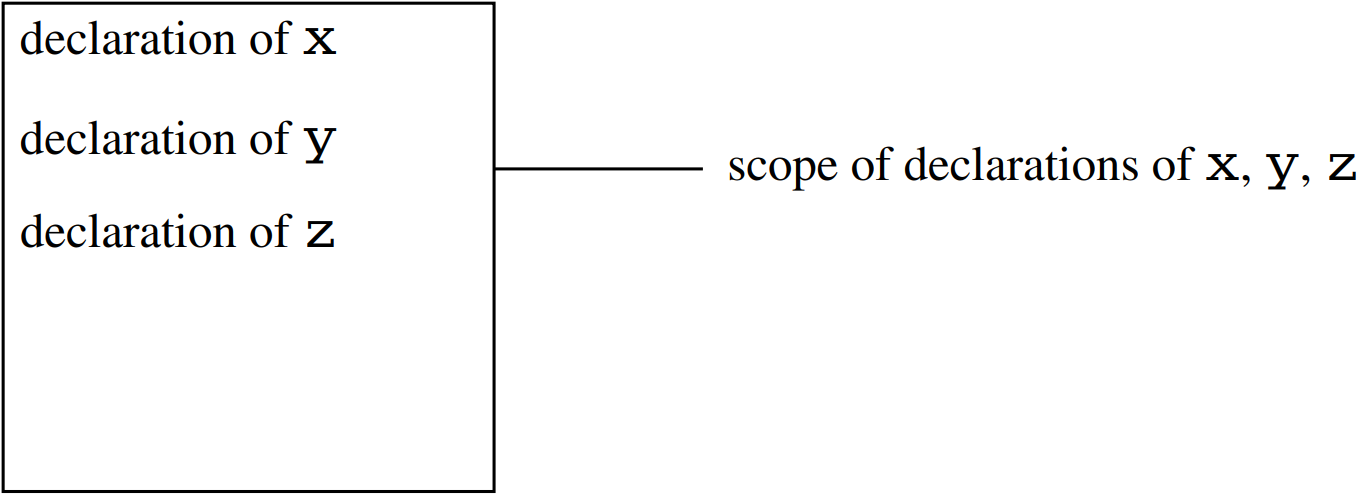
\includegraphics[width=\linewidth]{img/fig-4.1.png}
  \caption{Monolithic block structure.}
  \label{fig:fig1}
\end{figure}
In a long program with many identifiers, they share the same scope and they need to be distinct.

\subsubsection{Flat Block Structure}

In a language with \textit{\textbf{flat block structure}}, the program is partitioned into several non-overlapping blocks. In other words, program contains \textit{the global scope and only a single level local scope of function definitions}. No further nesting is possible.

\begin{figure}[H]
  \centering
  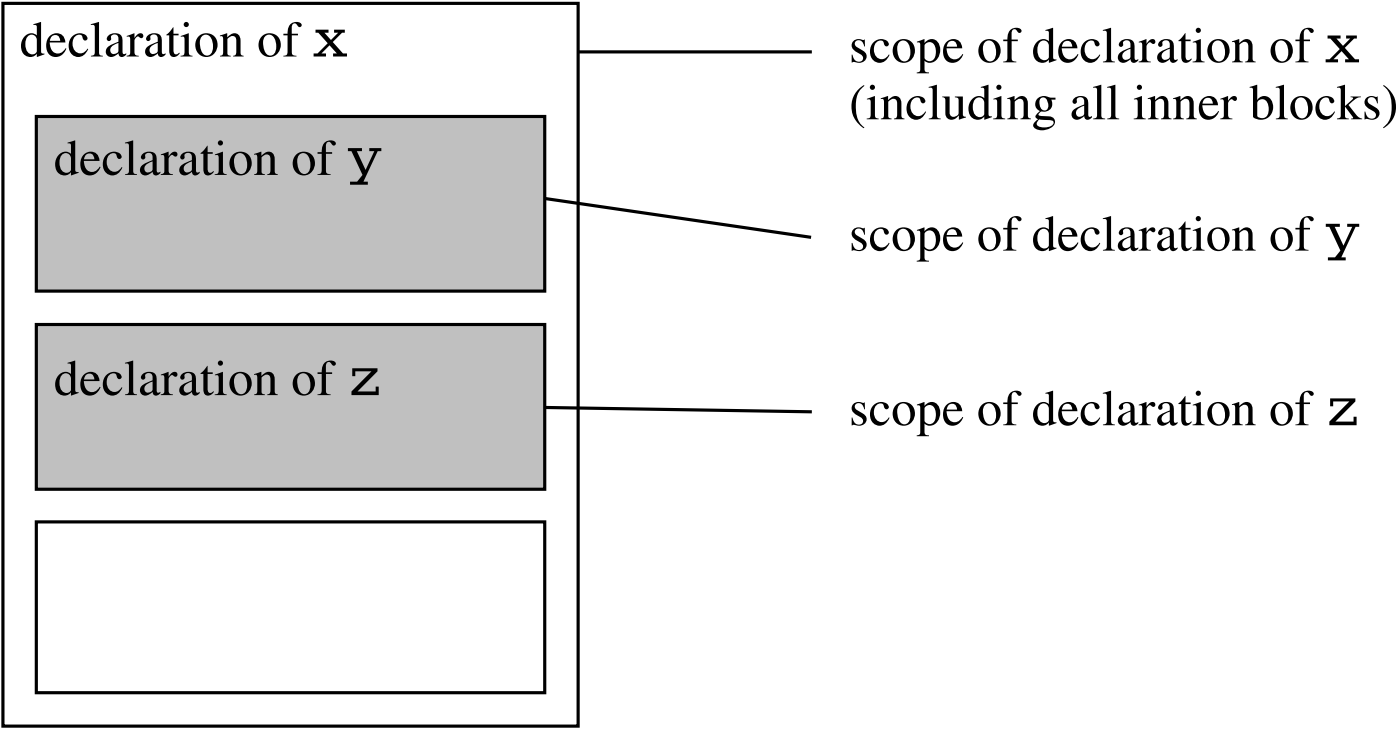
\includegraphics[width=\linewidth]{img/fig-4.2.png}
  \caption{Flat block structure.}
  \label{fig:fig2}
\end{figure}

\subsubsection{Nested Block Structure}

In a language with \textit{\textbf{nested block structure}}, blocks may be nested within other blocks.

\begin{figure}[H]
  \centering
  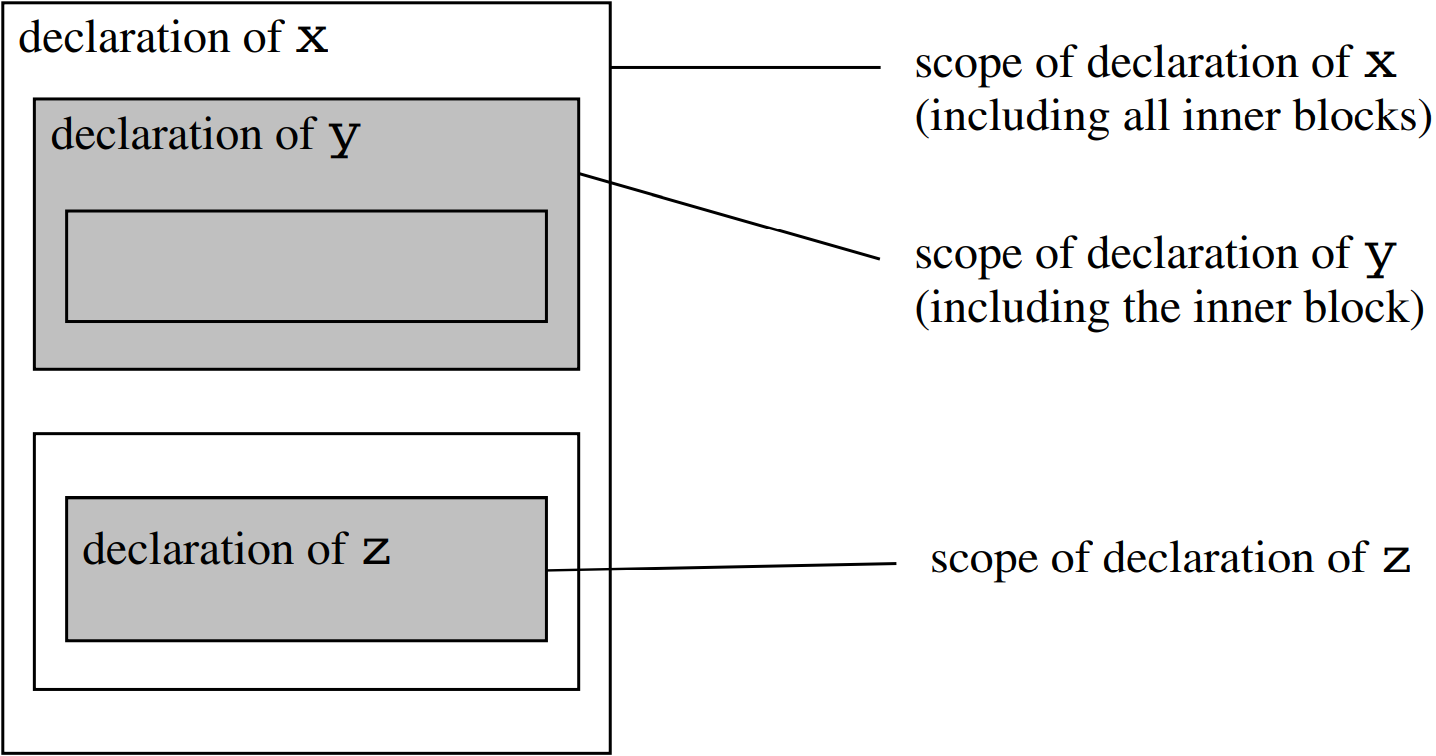
\includegraphics[width=\linewidth]{img/fig-4.3.png}
  \caption{Nested block structure.}
  \label{fig:fig3}
\end{figure}


\subsection{Scope and Visibility}

Consider all the occurrences of identifiers in a program. We must distinguish two different kinds of identifier occurrences:
\begin{itemize}
  \item A \textit{\textbf{binding occurrence}} of identifier \textit{I} is an occurrence where \textit{I} is bound to some entity \textit{X}.
  \item An \textit{\textbf{applied occurrence}} of \textit{I} is an occurrence where use is made of the entity \textit{X} to which \textit{I} has been bound. At each such applied occurrence we say that \textit{I} denotes \textit{X}.
\end{itemize}

When a program contains more than one block, it is possible for the same
identifier \textit{I} to be declared in different blocks. In general, \textit{I} will denote a different entity in each block.

Consider two nested blocks, such that the inner block lies within the scope of a declaration of identifier \textit{I} in the outer block:
\begin{itemize}
  \item If the inner block \textit{does not} contain a declaration of \textit{I}, then applied occurrences of \textit{I} both inside and outside the inner block correspond to the same declaration of \textit{I}. The declaration of \textit{I} is then said to be \textit{\textbf{visible}} throughout the outer and inner blocks.
  \item If the inner block \textit{does} contain a declaration of \textit{I}, then all applied occurrences of \textit{I} inside the inner block correspond to the inner, not the outer, declaration of \textit{I}. The outer declaration of \textit{I} is then said to be \textit{\textbf{hidden}} by the inner declaration of \textit{I}.
\end{itemize}

\begin{listing}[H]

\begin{minted}{c}
int x, y;

int f(double x) {
  ...             // parameter x hides global x
                  // in f()
}

int g(double a) {
  int y;         // local y hides global y in g()
  double f;      // local f hides global f()
                 // in g()
  ...
}

int main() {
  int y;        // local y hides global y
                // in main()
}
\end{minted}
\caption{}
\label{code:code4}
\end{listing}

\newpage

\end{multicols*}

\begin{multicols}{2}
\setlength{\columnsep}{1.5cm}
\setlength{\columnseprule}{0.2pt}

\subsection{Static vs Dynamic Scoping}

When are the binding and scope resolution done? In compile time or run
time? Two options:
\begin{enumerate}
  \item Static binding, static scope
  \item Dynamic binding, dynamic scope  
\end{enumerate}

The first defines scope and binding based on the lexical structure of the program and binding is done \textit{at compile time}. Second activates the definitions in a block during the execution of the block. The environment changes dynamically \textit{at run time} as functions are called and returned.

\vspace*{\fill}
\columnbreak

\subsubsection{Static Binding}

Programs' shape is significant. Environment is based on the position in the source (lexical scope). Most languages apply static binding (\texttt{C, Haskell, Pascal, Java, ...})

\begin{dummyenv}
\def\X{\color{green!60!black}\bf x}
\def\gX{\color{red!60!black}\bf x}
\def\Y{\color{green!60!black}\bf y}
\def\mY{\color{red!60!black}\bf y}
\def\fY{\color{yellow!60!black}\bf y}
\def\gA{\color{yellow!60!black}\bf a}
\def\mA{\color{red!60!black}\bf a}
\lstset{language=C,
        basicstyle=\footnotesize\ttfamily,
        keywordstyle=\color{blue!50!black}\bfseries,
        identifierstyle=\color{blue!60!green}\sffamily,
        stringstyle=\color{red!70!green}\ttfamily,
	      commentstyle=\color{blue!30!white}\itshape,
        showstringspaces=true}
\begin{listing}[H]
\begin{lstlisting}[language={C},escapechar=\#]
int #\X#=1,#\Y#=2;
int f(int #\fY#) {
      #\fY#=#\X#+#\fY#;     /* #\X# global, #\fY# local */
      return #\X#+#\fY#;
}
int g(int #\gA#) {
    int #\gX#=3;      /* #\gX# local, #\Y# global */
    #\Y#=#\gX#+#\gX#+#\gA#;    #\gX#=#\gX#+#\Y#;    #\Y#=f(#\gX#);
    return #\gX#;
}
int main() {
    int #\mY#=0;      /* #\X# global #\mY# local */
    int #\mA#=10;
    #\X#=#\mA#+#\mY#;    #\mY#=#\X#+#\mA#;    #\mA#=f(#\mA#);    #\mA#=g(#\mA#);
    return 0;
}
\end{lstlisting}
\caption{}
\label{code:code5}
\end{listing}
\end{dummyenv}

\end{multicols}

\subsubsection{Dynamic Binding}

Functions called update their declarations on the environment at run-time. Delete them on return. Current stack of activated blocks is significant in binding. \texttt{Lisp} and some script languages apply dynamic binding.

\begin{dummyenv}

% \noindent
\begin{minipage}[c]{0.35\textwidth}
%%%% Column 1 %%%%

\begin{listing}[H]

\begin{minted}[linenos]{c}
int x = 1, y = 2;

int f(int y) {
  y = x + y;      
  return x + y;
}

int g(int a) {
  int x = 3;       
  y = x + x + a; x = x + y;    
  y = f(x);
  return x;
}

int main() {
  int y = 0;  int a = 10;  
  x = a + y;  y = x + a;    
  a = f(a);   a = g(a);
  return 0;
}
\end{minted}
\caption{}
\label{code:code6}
\end{listing}

\end{minipage} %
\begin{minipage}[c]{0.65\textwidth}
%%%% Column 2 %%%%
\begin{dummyenv}
\def\T{\rule{0pt}{1em}\hspace*{1em}}
\noindent\normalsize\begin{tabular}{rll}
& Trace & Environment (without functions)\\ \hline
& initial & \{x:GL, y:GL \} \\ \rowcolor{blue!5}
12& call main & \{x:GL, y:main, a:main \} \\ \rowcolor{blue!15}
15&\T call f(10)  & \{x:GL, y:f , a:main \} \\ \rowcolor{blue!15}
4 &\T return f : 30 & back to environment before f  \\ \rowcolor{blue!5}
15& in main & \{x:GL, y:main, a:main \} \\ \rowcolor{blue!10}
15&\T call g(30) & \{x:g, y:main, a:g  \} \\ \rowcolor{blue!25}
9&\T\T call f(39) & \{x:g, y:f, a:g  \} \\ \rowcolor{blue!25}
4&\T\T return f : 117 & back to environment before f\\ \rowcolor{blue!10}
9&\T in g  & \{x:g, y:main, a:g  \} \\ \rowcolor{blue!10}
10&\T return g : 39 & back to environment before g \\ \rowcolor{blue!5}
15& in main & \{x:GL, y:main, a:main\} \\ \rowcolor{blue!5}
16& return main & x:GL=10, y:GL=2, y:main=117, a:main=39 \\
\end{tabular}
\end{dummyenv}

\end{minipage}

\end{dummyenv}

\begin{multicols*}{2}
\setlength{\columnsep}{1.5cm}
\setlength{\columnseprule}{0.2pt}


\end{multicols*}

\section{Binding Process}
\label{sec:binding-process}

Language processor keeps track of current environment in a data structure called \textit{\textbf{Symbol Table}} or \textit{\textbf{Identifier Table}}. Symbol table maps identifier strings to their type and binding. Each new block introduces its declarations/bindings to the symbol table and on exit, they are cleared. Usually implemented as a \textit{Hash Table}.

For static binding, Symbol Table is a compile time data structure and maintained during different stages of compilation. For dynamic binding, symbol table is maintained at run time.

\newpage

\begin{multicols*}{2}
\setlength{\columnsep}{1.5cm}
\setlength{\columnseprule}{0.2pt}


\section{Declaration}
\label{sec:declaration}

\textit{\textbf{Definition:}} Creating a new name for an existing binding.

\noindent \textit{\textbf{Declaration:}} Creating a completely new binding.

\begin{itemize}
  \item in \texttt{C}: \texttt{struct Person} is a declaration. \texttt{typedef struct Person persontype} is a definition.
  \item in \texttt{C++}: \texttt{double x} is a declaration. \texttt{double \&y=x;} is a definition.
\end{itemize}

The basic distinction is whether creating a new entity or not. However, usually the distinction is not clear and used interchangeably.

\subsection{Type Declaration}

A \textit{\textbf{type declaration}} binds an identifier to a type. We can distinguish two kinds of type declaration. A \textit{\textbf{type definition}} binds an identifier to an existing type. A \textit{\textbf{new-type declaration}} binds an identifier to a new type that is not equivalent to any existing type.

\subsection{Constant Declaration}

A \textit{\textbf{constant declaration}} binds an identifier to a constant value. A constant declaration typically has the form ``\texttt{const \textit{I} = \textit{E};}''.

\subsection{Variable Declaration}

A \textit{\textbf{variable declaration}}, in its simplest form, creates a single variable and binds an identifier to that variable. A \textit{\textbf{variable renaming definition}} binds an identifier to an \textit{existing} variable. In other words, it creates an \textit{alias}.

\subsection{Procedure Definitions}

A \textit{\textbf{procedure definition}} binds an identifier to a procedure. In most programming languages, we can bind an identifier to either a function procedure or a proper procedure.

\textit{Note: The following subsections are important.}

\subsection{Sequential Declarations}

A \textit{\textbf{sequential declaration}} composes subdeclarations that are to be elaborated one after another. Each subdeclaration can use bindings produced by any \textit{previous} subdeclarations, but not those produced by any \textit{following} subdeclarations.

Declared identifier is not available in preceding declarations but is available in following declaration.

Most programming languages provide only such declarations.

\subsection{Collateral Declarations}

A \textit{\textbf{collateral declaration}} composes subdeclarations that are to be elaborated independently of each other. These subdeclarations may not use bindings produced by each other. The collateral declaration merges the bindings produced by its subdeclarations.

Collateral declarations are uncommon in imperative and object-oriented languages, but they are common in functional and logic languages.

\subsection{Recursive Declarations}

A \textit{\textbf{recursive declaration}} is one that uses the bindings that it produces itself. Such a construct is important because it enables us to define recursive types and procedures.

\textit{Declaration:} \texttt{Name = Body}. The body of the declaration can access the declared identifier. Declaration is available in the body of itself.

\texttt{C} functions and type declarations are recursive. Variable definitions are usually not recursive.

\subsection{Recursive Collateral Declarations}

All declarations can access the others regardless of their order.
\begin{itemize}
  \item All \texttt{Haskell} declarations are recursive collateral (including variables). All declarations are mutually recursive.
  \item \texttt{C++} class members are like this.
  \item In \texttt{C}, a similar functionality can be achieved by prototype
  definition.
\end{itemize}

\subsection{Scopes of Declarations}

\textit{Collateral}, \textit{sequential}, and \textit{recursive declarations} differ in their influence on scope:
\begin{itemize}
  \item In a \textit{collateral declaration}, the scope of each subdeclaration extends from the end of the collateral declaration to the end of the enclosing block.
  \item In a \textit{sequential declaration}, the scope of each subdeclaration extends from the end of that subdeclaration to the end of the enclosing block.
  \item In a \textit{recursive declaration}, the scope of every subdeclaration extends from the start of the recursive declaration to the end of the enclosing block.
\end{itemize}


\newpage
\section{Blocks}
\label{sec:blocks}

If we allow a command to contain a local declaration, we have a \textit{block command}. If we allow an expression to contain a local declaration, we have a\textit{block expression}.

\subsection{Block Commands}

A block command is a form of command that contains a local declaration (or group of declarations) \textit{D} and a subcommand \textit{C}. The bindings produced by \textit{D} are used only for executing \textit{C}.

In other words, declarations done inside a block command is available only during the block. Statements inside work in this environment. The declarations lost outside of the block.

\begin{listing}[H]
\begin{minted}{c}
int x = 3, i = 2;
x += i;
while (x > i) {
  int i = 0;
  ...
  i++;
}
/* i is 2 again */
\end{minted}
\caption{}
\label{code:code7}
\end{listing}


\subsection{Block Expressions}

A \textit{\textbf{block expression}} is a form of expression that contains a local declaration (or group of declarations) \textit{D} and a subexpression \textit{C}. The bindings produced by \textit{D} are used only for evaluating \textit{E}.

In other words, it allows an expression to be evaluated in a special local environment. Declarations done in the block is not available outside.

\begin{listing}[H]
\begin{minted}{Haskell}
x=5
t=let xsquare=x*x
      factorial n = if n<2 then 1
                    else n*factorial (n-1)
      xfact = factorial x
  in  (xsquare+1)*xfact/(xfact*xsquare+2)
\end{minted}
\caption{}
\label{code:code8}
\end{listing}

\vspace*{\fill}
\columnbreak

\noindent Hiding works in block expressions as expected:
\begin{listing}[H]

\begin{minted}{Haskell}
x=5 ; y=6 ; z = 3
t=let x=1 
  in let y=2 
     in   x+y+z
{--
t is 1+2+3 here. 
local x and y hides the ones above
--}
\end{minted}
\caption{}
\label{code:code9}
\end{listing}

\noindent GCC (only GCC) block expressions has the last expression in block as the value:
\begin{listing}[H]

\begin{minted}{c}
double min ;
...
min =  ({ double tmp;
          if (b < a) then {
            tmp = a;  a = b ; b = tmp;
          }
          a; // this is the value of the block
        });
\end{minted}
\caption{}
\label{code:code10}
\end{listing}

\subsection{Block Declaration}

A declaration is made in a local environment of declarations. Local declarations are not made available to the outer environment.

In \texttt{Haskell}: \texttt{D$_{exp}$ where D$_1$; D$_2$;  ... ; D$_n$}

\noindent Only \texttt{D$_{exp}$} is added to environment. Body of \texttt{D$_{exp}$} has all local declarations available in its environment.

\begin{listing}[H]

\begin{minted}{Haskell}
fifthpower x = (forthpowerx) * x where
               squarex = x*x;
               forthpowerx = squarex*squarex
\end{minted}
\caption{}
\label{code:code11}
\end{listing}





\end{multicols*}

\end{document}
